\section{Introduction}

\begin{figure*}[t]
    \centering
    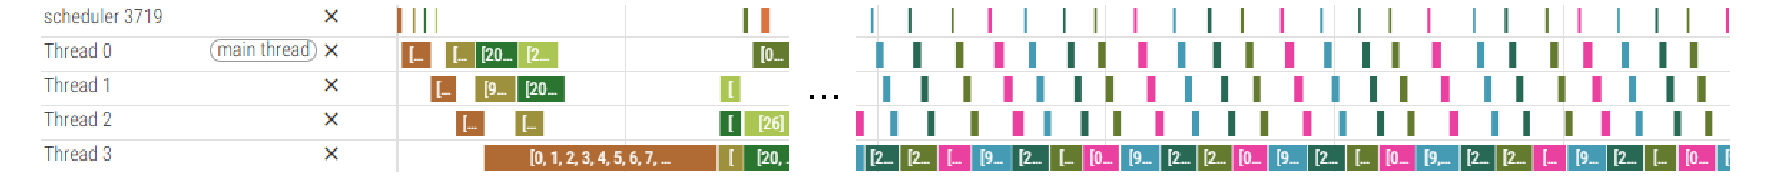
\includegraphics[width=1\linewidth]{figures/trace_lyz_new_new.pdf}
    \caption{An LLM pipeline timeline generated by Perfetto. 
    The data is taken on a system with  4 RTX 3090 GPUs running a four-stage pipeline using the ShareGPT dataset. The different colored blocks represent different batches on each thread running on a GPU, while the white areas indicate pipeline bubbles. It shows that the bubbles begin to emerge and persist after the first few batches due to the limited memory capacity.
    }
    \label{trace}
\end{figure*}

Large Language Models (LLMs) have emerged as a cornerstone of artificial intelligence, demonstrating remarkable applicability to many domains. Significant progress has been reported in code generation\cite{mathews2024test}, text translation\cite{dabre2020survey}, dialogue systems\cite{roller2021recipes} and other applications\cite{lee2024infinigen}. 
To meet increasingly complex application requirements, enhancing the capabilities of LLMs is critical. 
Scaling up the model size has been identified as an effective strategy to achieve this objective\cite{koto-etal-2023-indommlu}. 
Consequently, the size of LLMs has grown exponentially\cite{10549890}, resulting in substantial improvements in their capability and performance. For instance, Llama2-70B exhibits a 42\% improvement in solving mathematical problems compared to its smaller counterpart, Llama2-7B\cite{koto-etal-2023-indommlu}.

As the model size increases, the demand for memory and computational resources also grows, often surpassing the capacity of the host device. 
To address this challenge, employing multi-device clusters for parallel inference and fully leveraging their capabilities have become a key strategy to improve performance.
% rebuttal: 补充是否添加tp
Among various parallel inference techniques, \emph{pipeline parallelism} is a commonly used approach. Technologies such as Google's Gpipe\cite{huang2019gpipe}, Microsoft's DeepSpeed\cite{aminabadi2022deepspeed}, and Nvidia's TensorRT\cite{davoodi2019tensorrt} all leverage pipeline-based parallel inference.
This technology divides the LLM layers into multiple pipeline stages. Each stage is assigned to a separate GPU, thus enables parallel execution across stages. It can significantly enhance the inference throughput and support efficient deployment of LLM.

To fully utilize device resources, the LLM inference engines employ iteration-level schedulers \cite{yu2022orca}, which enhance parallelism by batching tasks at the token-level granularity. 
These advancements mitigate some of the impact caused by the pipeline bubbles and significantly improve the performance, contributing to their widespread adoption \cite{patel2024splitwise, jin2023s, qin2024mooncake}. 
Leading inference frameworks, such as DeepSpeed \cite{aminabadi2022deepspeed}, vLLM \cite{kwon2023efficient}, have integrated such batching techniques.




However, we have observed that this batching cannot fully eliminate the pipeline bubbles. 
We measure GPU utilization using a four-stage pipeline running the workload of the ShareGPT dataset\cite{chiang2023vicuna}. 
The results visualized by Perfetto\cite{perfetto2021} are shown in Figure \ref{trace}.  
There are 4 threads: Threads 0 to 3 with Thread 0 as the Main Thread, each thread on one GPU.
The x-axis shows the elapsed running time.
The figure shows that GPUs are fully utilized only in the first iteration of the inference task, i.e., there is no white space in that period of elapsed time for all threads.
As the inference progresses, pipeline bubbles begin to emerge and persist, shown as white spaces between colored fragments in Threads 0, 1, and 2. Each green fragment represents the execution time for one stage of the inference in a batch running on that thread.
In this scenario, GPUs spend approximately \textbf{60\%} of the time in the stalled state due to the pipeline bubbles. 



A more detailed analysis reveals that this issue is inherent to pipeline-based approaches. 
The primary cause is the mismatch between computational and memory resources in GPUs. 
As illustrated in Figure~\ref{trace}, the formation of bubbles in Threads 0, 1, and 2 is attributed to GPU memory being fully committed.
It prevents the scheduler from assembling new batches until after the completion of the last stage of the previously launched batch. 
It leaves the GPUs for Threads 0,1,2 waiting in an idle state.
Only Thread 3 is fully committed because there is additional computation workload in the last stage of token generation inference, such as projection and token sampling.
This phenomenon highlights a fundamental limitation of the pipeline design, which we will explore further in Section~\ref{sec:pipelinebubble}.

Moreover, although GPUs are idle during the stalled state, they nevertheless continue to draw substantial amounts of power, resulting in unnecessary waste.
Energy efficiency is a critical issue that has garnered significant attention from both academia and industry. 
Existing LLM systems have highlighted such energy efficiency challenges. 
For example, estimates from \cite{patterson2021carbon} indicate that training the GPT-3 model requires 1,287 MWh of energy, equivalent to the annual energy consumption of 420 individuals. 
The energy demands during LLM inference are also noteworthy. Each ChatGPT inference, for instance, consumes approximately 2.9 watt-hours (Wh) of electricity, nearly ten times the 0.3 Wh used by a single Google search\cite{shi2024efficient}.


% Various techniques have been proposed and employed to mitigate the high power and energy usage associated with LLM workloads. 
% For example, NVIDIA GPUs can  adjust power using the \emph{dynamic voltage and frequency scaling (DVFS)} to decrease or increase power ratings based on the workload demands \cite{nvidia}. 
% Existing application-level interfaces on GPUs also support effective software-guided power and energy management. 
% However, due to the overhead of monitoring workload fluctuation and the required latency in power adjustments at runtime, these mechanisms usually operate at the rates of seconds and  with power changes at even longer intervals \cite{chen2023joss}.
% In contrast, each pipeline bubble  typically persists for only a few milliseconds. 
% The coarse resolution prevents most existing schemes from effectively detecting and responding to such brief workload fluctuations, rendering them inadequate for managing power and energy changes in this context.

% Various techniques have been proposed and employed to mitigate the high energy comsumpation while not affecting the performance. 
% 硬件层面，英伟达GPU能够自动检测任务负载的变化，从而动态调节GPU的电压和频率(DVFS)
% 用户层面，人工可以通过NVML指令动态调节GPU的频率，降低位于非critical-path上的computation的频率，实现节能的效果。
% 然而，GPU频率调节的时间粒度是几个到几十个milliseconds，which 和气泡的时间相等 during inference。
% 这使得it hard to 动态调节频率来消除bubble处的能耗
% \bylyz{
Various techniques have been proposed to optimize energy efficiency in LLM workloads without compromising performance.
NVIDIA GPUs can autonomously detect workload fluctuations and dynamically modulate power via dynamic voltage and frequency scaling (DVFS)~\cite{nvidia}. 
ThrottLL'eM~\cite{kakolyris2025throttll} analyzes the impact of GPU frequency on LLM  energy efficiency, employing dynamic frequency scaling informed by environmental factors to enhance efficiency. 
Perseus~\cite{chung2024reducing} dynamically lowers frequencies for non-critical-path computations to mitigate energy consumption through manual frequency adjustments. 
Nonetheless, the overhead of these GPU adjustment mechanisms ranges from several to tens of milliseconds~\cite{chen2023joss}, a timescale commensurate with the duration of pipeline bubbles during inference. 
This equivalence renders dynamic GPU regulation ineffective for decreasing energy waste within these bubbles.
% }



To address these issues, we propose a counterintuitive strategy.
% Instead of using DVFS to lower power when bubbles occur, we reduce the GPU’s \textit{frequency} (the configurable upper bound on its power consumption) to slow computation, thereby preventing bubble formation. 
\bylyz{
Instead of dynamically setting the frequency when bubble occur, we staticly reduce the GPU's frequency to slow computation, thereby preventing bubble formation. 
As discussed earlier, bubbles in Threads 0, 1, and 2 arise from a mismatch between GPU compute and memory resources. 
In our proposed approach, instead of using full frequency to process the required stage of a batch and then wait for memory resources to become available for the next batch (i.e., to form a bubble), we intentionally lower the frequency to slow down the computation of each batch, which can then match the time when memory resource is released and becomes available.
}


Ideally, if the completion time of the first stage in the current batch is delayed sufficiently to align with the finish time of a previously launched batch in the last stage, no pipeline bubbles will form. 
As a batch finished, the scheduler can initiate the construction of a new batch in time.
The alignment ensures that the subsequent inference batch is ready just as Thread 0 completes its current batch, i.e. eliminating the bubbles on Thread 0.
Additionally, the extended execution time of stages across multiple batches enables them to be more closely connected, reducing bubbles between stages, as the colored fragments in Figure \ref{trace} will be extended to replace the white space following them.
Such frequency adjustments are much more manageable because they are at a coarser grain (i.e., applied to all colored fragments) than that of individual bubbles (more details in Section~\ref{sec:pipelinebubble}).


To reduce these bubbles during inference presents several challenges.
\bylyz{
First, the optimal GPU frequency must be determined within a minimal profiling time to maintain low overhead. 
Second, the targeted frequency configuration must be highly precise to maximize bubble reduction without compromising inference performance.
Third, the framework should possess broad generalizability across diverse hardware platforms and various pipeline-parallel LLM architectures.
}

% \bygpt{
% Reducing pipeline bubbles during inference through static GPU frequency adjustment presents three challenges.
% First, suitable frequencies must be identified with low tuning overhead.
% Second, the selected frequencies must be based on accurate estimates of stage execution time, allowing faster stages to exploit available pipeline slack while limiting performance degradation.
% Third, the framework should be applicable across different hardware platforms and LLMs deployed with pipeline parallelism.
% }
% First, high-resolution power scaling is not available. 
% Current GPU power management cannot operate at the level of milliseconds required to respond to individual pipeline bubbles effectively. 
% This limitation is primarily due to the inherent latency of power-scaling operations and the constraints of existing hardware and firmware designs\cite{chen2023joss}.
% Second, accurately controlling the execution time of LLM inference to prevent the formation of bubbles by power scaling is non-trivial. 
% Third, the proposed framework should be general and applicable to different machine platforms and different pipeline-based LLM models.


% To tackle these challenges, we quantify the relationship between iteration-level batch latency and the GPU’s power rating for a given model. 
% Although input data might seem to influence iteration latency, we find it is largely determined by the model’s configuration and power setting, \bygxl{due to the heavy computation over fixed model parameters}(more details are discussed in Section~\ref{sec:stableexecutiontime}). 
% \bygxl{!!!REWrite this paragraph!!!Although input data might seem to influence iteration latency, we find it is largely determined by the model’s configuration and power setting, due to the advancements in long-context processing optimizations and heavy computation over fixed model parameters (more details are discussed in Section~\ref{sec:stableexecutiontime}).} 
% However, the batch lantency is also influenced by the 这个batch中的sequence length和batchsize，which is hard to predict and control during the iteration.
% However, we found the impact is negligible during the decode phase, where we focused, due to the advancements in long-context processing optimizations and heavy computation over fixed model parameters (more details are discussed in Section~\ref{sec:stableexecutiontime}).
% \bylyz{Although batch latency is also theoretically influenced by sequence length and batch size which are hard to predict and controlled during the runtime, we find their impact to be negligible during decoding phase where we focus, due to  advances in long-context optimization and the dominant cost of computations over fixed model parameters (more details are discussed in Section~\ref{sec:stableexecutiontime}).}
% Leveraging this input-insensitive property, we build an analytical model through one-time profiling of a small set of batched iterations in a pipeline-parallel LLM. 
% This model enables the host GPU to set power ratings that align stage completion times and eliminate pipeline bubbles.

To address these challenges, we conduct a thorough study on the behavior of the LLM inference tasks.
Firstly, we find that the iteration-level batch execution time of a given model during LLM inference is stable and largely input-insensitive, as it is dominated by the model’s heavy parameter loading and high parallel computation capacity(see Section~\ref{sec:stableexecutiontime}). 
Based on this observation,  an analytical model can be established by one-time profiling of a limited number of batched iterations in a pipeline-based LLM model.
This model provides actionable guidance to set the frequency of GPUs and effectively reduce pipeline bubbles. 



In this paper, we propose \thisproj{}, a general framework that regulates GPU frequency to optimize energy efficiency in pipeline-based LLM inference engines.
We develop an analytical model capturing the relationship between GPU frequency and execution time of stages in the LLM pipelines. 
Guided by this model, \thisproj{} reduces pipeline bubbles, enabling significant power efficiency improvements with minimal performance impact.
We have proved the effectiveness of \thisproj{} on both \hcwplaceholder{XXX} and \hcwplaceholder{XXX} and our experiments show up to \hcwplaceholder{XX}\% energy efficiency improvement, with average improvements of \hcwplaceholder{XXX}\% on Llama3-8B and \hcwplaceholder{XXX}\% on Llama3-70B.
In summary, we make the following contributions.

\begin{itemize}
\item 
We analyze iteration-level batch inference in pipeline-parallel LLMs, showing that inevitable bubbles arise from stage execution time misalignment caused by compute–memory mismatches. 
We further demonstrate that stage execution times are largely input-insensitive, offering opportunities for optimization.

\item We propose \thisproj{}, an LLM inference optimization framework that reduces pipeline bubbles through model-guided static frequency adjustments.
It constructs a quantitative analytical model, leveraging input-insensitive execution time characteristics, to describe the relationship between energy efficiency and performance based on offline, one-time profiling.
The approach is general and effective across diverse LLM inference engines.

\item We have implemented \thisproj{} for state-of-the-art pipeline-based LLM inference engines using continuous batching \cite{yu2022orca}. 
Extensive experiments demonstrate that \thisproj{} improve energy efficiency by up to \hcwplaceholder{XXX}\%, with an average reduction of \hcwplaceholder{XXX}\% on Llama3-8B and \hcwplaceholder{XXX}\% on Llama3-70B, al  l while maintaining the inference engine's high performance.
\end{itemize}


The rest of the paper is organized as follows. Section~\ref{sec:background} provides necessary background about LLM inference.
Section~\ref{sec:design} presents the design and implementation of \thisproj{}. 
Section~\ref{sec:evaluation} evaluates \thisproj{} with various benchmarks and discussed the experimental results. 
% Then, Section~\ref{sec:relatedworks} discussed some other works related to our work. 
% Section~\ref{sec:discussion} discusses our work's applicability and limitations
Section \ref{sec:relatedworks} reviews related work.
Section \ref{sec:discussion} discusses the applicability and limitations of our approach.
Finally, section \ref{sec:conclusion} concludes the paper.





